%%
%% Template intro.tex
%%

\chapter{Introduction}
\label{cha:intro}

\section{Description}

Finding relevant information from the glut of data is one of the biggest challenges faced by users today. This is important not just for the users themselves, but also for companies that may wish to sell or provide a service to them. One way to help users find relevant information is through automatic recommender systems. Recommender systems seek to automatically discover what the user's preferences are.

\subsection{Individual Recommendation}

Individual recommendation models a user's preferences through information about the user alone. This information can be the user's profile details like age, sex, and occupation, as well as the user's history like previously bought or rated items.

\subsection{Collaborative Recommendation}

Collaborative recommendation models a user preferences not just through information about the user alone, but also through information about the other users. Collaborative recommendation algorithms examples are k-nearest neighbors and probabilistic matrix factorization.

\subsection{Social Recommendation}

In contrast to collaborative recommendation, which treats all users as equal for recommendation, social recommendation makes use of certain links to help calculate similarity between users. Additional information help with recommendation. It has been shown that users are more likely to have the same preference with their friends than with other random users.

These links could be connections between users in social networks like Facebook and MySpace, or some other measure of user interaction and similarity.

\section{Facebook}

Facebook is a social networking service that is currently the largest in the world. As of July 2011 it has more that 750 million active users. Users in Facebook create a profile and establish "friend" connections between users to establish their social network. Each user has a "wall" where they and their friends can make posts to. These posts can be links, photos, status updates, etc. Items that have been posted by a user can be "liked", shared, or commented upon by other users. 

\begin{figure}[h]
\centering
\subfigure{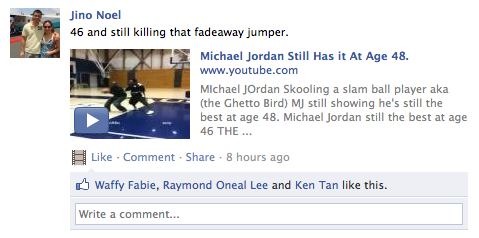
\includegraphics[scale=0.50]{img/posted-link.png}}
\caption{A link posted by the author that has been liked by three other users.}
\end{figure}

This paper seeks to find out how best to recommend links to individual users such that there is a high likelihood of them "liking" it. We do this by creating a Facebook application that recommends links to users everyday and the users could give their feedback on the links, whether they liked it or disliked it. 

\section{LinkR}
Facebook allows applications to be developed that can be installed by their users. As part of this project, the LinkR Facebook application was developed. The functionalities of the LinkR application are:

\begin{enumerate}
\item{Collect data that have been shared by users and their friends on Facebook.}
\item{Recommend links to the users daily.}
\item{Collect feedback from the users on whether they liked or disliked the recommendations.}
\end{enumerate}

\begin{figure}[h]
\centering
\subfigure{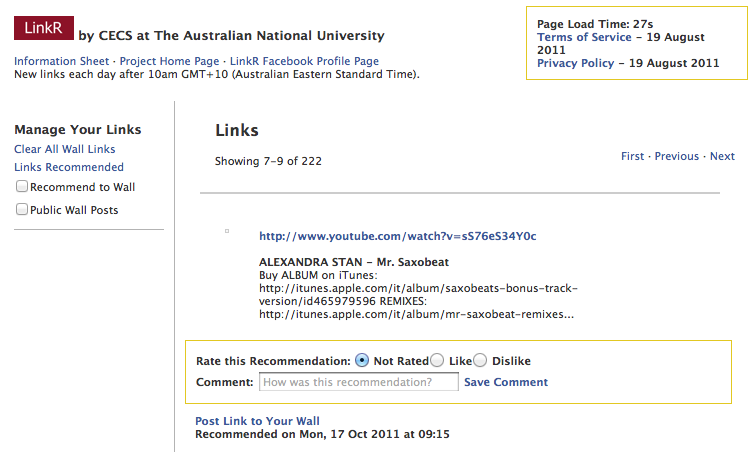
\includegraphics[scale=0.30]{img/linkr.png}}
\caption{The LinkR application showing one of the recommendations.}
\end{figure}

The main developer of LinkR is Khoi-Nguyen Tran, a PhD student at the Australian National University. The algorithms it uses at the backend for recommendation was developed as part of this paper. 


\section{Chapter Outline}

In the following chapters we will show that social information can be an effective tool that can be used to improve recommender systems. In Chapter 2 I  discuss the background of the project, the notations, evaluation metrics, description of algorithms, as well as other resources that were used for this paper.

In Chapter 4  I discuss and compare various social and non-social recommendation algorithms and run them on a Facebook dataset that was compiled as part of this project. I also discuss preliminary results of the bigger Facebook project that this paper is a part of.

In Chapter 5 I give my conclusions from my work and future directions that this research could go to.


%%% Local Variables: 
%%% mode: latex
%%% TeX-master: "thesis"
%%% End: 
